\usepackage[authoryear,round]{natbib}
\usepackage{multirow}

\newcommand{\sheetnum}{%
	14
}
%\setcounter{section}{\sheetnum-3}
\newcommand{\tutorialtitle}{%
    Reinforcement Learning Pt 1/2 
    (Value estimation)
}
\newcommand{\tutorialtitleshort}{%
	RL (Value estimation)
}
% for slides
\subtitle{\sheetnum \tutorialtitle}

\maxdeadcycles=1000 % Workaround for ! Output loop---100 consecutive dead cycles because of too many figures

% The following use of algroithms does not work well with the notes:
%
%
%
%
% instead use the following for your algorithms:
%
%\begin{figure}[!t]
%\removelatexerror
%\begin{algorithm}[H]
    % your algo here
    %\label{alg:algolabel}
    %\caption{algocaption}
%\end{algorithm}
%\end{figure}
%\begin{algorithm}
% Below is the definition for the command \removelatexerror:
\makeatletter
\newcommand{\removelatexerror}{\let\@latex@error\@gobble}
\makeatother

\begin{document} %%%%%%%%%%%%%%%%%%%%%%%%%%%%%%%%%%%%%%%%%%%%%%%%%%%%%%%

\sheet{\sheetnum}{\tutorialtitleshort}

\ttopic{\tutorialtitle}

\columnratio{0.2,0.8}\textbf{}
\begin{paracol}{2}
%\setlength{\columnseprule}{0.1pt}
%\setlength{\columnsep}{5em}

\begin{rightcolumn}

% notes version will ignore it
\begin{frame}
\titlepage
\end{frame}

\begin{frame}
\tableofcontents[hideallsubsections]
\end{frame}

\mode<all>
\section{The Reinforcement Learning (RL) setting}


\definecolor{reward}{rgb}{0,0.5,0}
\definecolor{policy}{rgb}{0.75,0,0}
\definecolor{trans}{rgb}{0,0,1}

\begin{frame}\frametitle{\secname}

\only<1>{
Reminder:
\begin{itemize}
\item Data in supervised learning:
$
\Big\{
	\vec x^{(\alpha)} \in \R^N
	\,,\,
	\vec y_T^{(p)} \in \R^M
\Big\}_{\alpha=1}^{p}
$

\item Data in \textbf{un}supervised learning:
$
\Big\{
	\vec x^{(\alpha)} \in \R^N
\Big\}_{\alpha=1}^{p}
$\\

\end{itemize}
}

\only<1->{
Data in Reinforcement Learning:
}
\only<1>{
\begin{itemize}
	\item[] A sequence of random states $\vec x$
	\item[] resulting from taking actions $\vec a$ over time
	\item[] which result in some reward $r$.
\end{itemize}
}
\pause
\only<2->{
\begin{itemize}
\item a state $\vec x \in \mathcal{X}$ or $\vec x \in \R^N$,\\
e.g. $\mathcal{X} := \{ \vec x_1, \ldots, \vec x_S\} \subset \{0,1\}^S$ (1-out-$S$ encoding)
\pause
\item an action $\vec a$ which can be taken by the agent:\\

$\vec a \in \mathcal{A}$ or $\vec a \in \R^M$,\\
 e.g. $\mathcal{A} := \{ \vec a_1, \ldots, \vec a_A\} \subset \{0,1\}^A$ (1-out-$A$ encoding)
\pause
\item a reward $r \in \R$ or $r \in \{0,1\}$,\\
 e.g. $r \in \{\text{``cheese''},\text{``no cheese''}\}$.

\end{itemize}
\pause
\mode<article>{Each time step describes what reward was received when performing some action while in some state. 
}
The sequence we observe becomes:

\slidesonly{\vspace{-4mm}}

\begin{align}
\label{eq:chain}
\left\{\vec x^{(t)}, \vec a^{(t)}, r^{(t)}\right\}_{t=0}^{p} = 
\left( \vec x^{(0)}, \vec a^{(0)}, r^{(0)} \right) \,,\, \ldots \,,\, \left(\vec x^{(p)}, \vec a^{(p)}, r^{(p)} \right)
\end{align}
}

\end{frame}

\subsection{The Transition Model}

\begin{frame}

\only<1,2>{    
\begin{block}{Markov property}

The probability of transitioning from state $\vec x_i$ to $\vec x_j$ only depends on state $\vec x_i$ and the action $\vec a_k$ that was taken. It does not depend on earlier history.
\end{block}
}
\only<2-4>{
This leads to the following \textcolor{trans}{transition model (transition ``matrix'')}:

\svspace{-3mm}

\begin{equation}
{
\color{trans}
P(\vec x_j | \vec x_i, \vec a_k)
}
\end{equation}

\only<2->
{
which
\begin{itemize}
	\item measures the probability to end up in $\vec x_j$ 
		after choosing $\vec a_k$ when in $\vec x_i$,
	\item is a stationary distribution
	\begin{equation}
	P(\vec x_j^{(t+1+\tau)} | \vec x_i^{(t+\tau)}, \vec a_k^{(t+\tau)}) = P(\vec x_j^{(t+1)} | \vec x_i^{(t)}, \vec a_k^{(t)})\,,\quad \tau \in \{0,1,\ldots\}
	\end{equation}
\end{itemize}
}
\only<3>{
\mode<presentation>{
	\begin{center}
		
\includegraphics[width=0.3\textwidth]{img/meme_stationary}
	\end{center}
	}
}
\only<4>{

and where
\begin{align}
{\color{trans}P(\vec x_j | \vec x_i, \vec a_k)} &\ge 0 \quad \forall i,j,k\\
\text{and}~ \sum_{j} {\color{trans}P(\vec x_j | \vec x_i, \vec a_k)} &= 1 \quad \forall i,k \quad \text{i.e. every ``row'' sums to 1}
\end{align}
}
}

\end{frame}

\begin{frame}{Properties of the transition model}

\svspace{-4mm}

\question{What would $\sum_{\substack{j\\j \ne i}} {P(\vec x_j | \vec x_i, \vec a_k)} = 0 \;\; \forall \; k$ imply?}

\pause

\slidesonly{\vspace{-3mm}}
- $\vec x_i$ \notesonly{is a state which leads nowhere else, regardless of the action. It }is a \emph{terminal state}.

\question{What does an entry ${P(\vec x_j | \vec x_i, \vec a_k)} = 0$ represent?}

\pause

- When at $\vec x_i$, taking action $\vec a_k$ can never lead to $\vec x_j$.


\question{What does an entry ${P(\vec x_j | \vec x_i, \vec a_k)} = 0 \;\; \forall \; k$ represent?}

\pause

- It is impossible to go from $\vec x_i$ to $\vec x_j$, regardless of the action.

\question{What does an entry ${P(\vec x_j | \vec x_i, \vec a_k)} = 1$ represent?}

\pause

- When at $\vec x_i$, taking action $\vec a_k$ always leads to $\vec x_j$.

\end{frame}

\begin{frame}

\mode<presentation>{
\textcolor{trans}{transition model (transition matrix)}:

\begin{equation}
{
\color{trans}
P(\vec x_j | \vec x_i, \vec a_k)
}
\end{equation}
}

\begin{block}{Markov chain}
a sequence of random states $\vec x$ with a \emph{Markov property}.
\end{block}


\end{frame}

\subsection{The Policy}

\begin{frame}

\begin{block}{\textcolor{policy}{Policy}}
Representation of the agent\footnote{
Without a policy we would only have a Markov Reward Process.
Having a policy (wanting to find a policy) turns the Markov Reward Process into a Markov Decision Process.
}. It measures the distribution over actions given states.
\begin{itemize}
\item map states to actions, i.e. the probability of doing $\vec a_k$ when in $\vec x_i$:

\begin{equation}
\color{policy}
\text{policy }\pi := \pi(\vec a_k | \vec x_i)
\end{equation}

\pause

\item the mapping can be stochastic or deterministic
\item the policy is stationary. That the policy changes during the training process does not contradict this.
It is regarded as stationary because once trained and deployed, the way the agent decides does not change over time.
\end{itemize}

\end{block}

\end{frame}

\mode*

\clearpage

\mode<all>
\section{Markov Decision Process (MDP)}

\definecolor{darkgreen}{rgb}{0,0.6,0}

\begin{frame} 
\mode<presentation>{
    \begin{center} \huge
        \secname
    \end{center}
}
    \begin{center}
    A formalized description of the \underline{environment} in RL\footnote{Recommended reading 
\citep{sutton1998introduction} also video lectures by David Silver}
    \end{center}
\end{frame}


\begin{frame}\frametitle{\secname}
    
\begin{block}{Assumption of MDP}
The environment is fully observable. There is a complete characterization of what's going on and where everything is.
\end{block}

The other case would be \emph{partially observable} MDP (POMDP)

\end{frame}


\begin{frame}\frametitle{\secname}

\begin{block}{What do we want to do}
Maximize, not just immediate rewards but the \emph{cumulative sum of rewards} or ``return''.
\slidesonly{\vspace{-3mm}}
\begin{equation}
\mathit{return}(t) := \sum_{k=0}^{\infty} \gamma^k r(\vec x^{(t+k+1)}, \vec a^{(t+k+1)}) = \sum_{k=0}^{\infty} \gamma^k r^{(t+k+1)},
\end{equation}

where $\gamma \in \lbrack0,1)$ is referred to as the \emph{discount factor}.
 
\end{block}

\only<1>{
About the \emph{discount factor} $\gamma$:
}

\begin{itemize}
\only<1>{
\item It is possible for $\gamma$ to be $=1$.\\

\question{Under what condition can $\gamma$ be $=1$}\\


\mode<article>{
- $\gamma$ can be $=1$ if the length of the sequence is guaranteed to be finite.
}
}

\pause

\item \question{What does $\gamma \rightarrow 0$ imply?}\\

- preference for short term rewards

\pause

\item \question{What does $\gamma \rightarrow 1$ imply?}\\

\pause

- emphasis on long-term returns, indifference to delay.

\end{itemize}

\end{frame}

\begin{frame}\frametitle{The discount factor}
 
\mode<presentation>{
\begin{equation}
\mathit{return}(t) := \sum_{k=0}^{\infty} \gamma^k r^{(t+k+1)},\quad \text{where }\gamma \in \lbrack0,1)
\end{equation}

}

\mode<article>{
\figref{fig:discount} illustrates how the choice of $\gamma$ controls how fast the discount factors decay over time.
}

\begin{center}
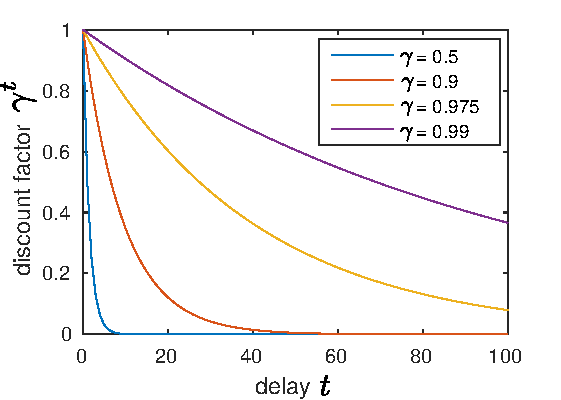
\includegraphics[width=6cm]{img/delay_discount}
\captionof{figure}{modulating returns with different discount factors}
\label{fig:discount}
\end{center}

\slidesonly{\vspace{-3mm}}
\slidesonly{\textbf{(see blackboard)}}

\mode<article>{

\newpage

\textbf{Example}: big reward further away vs. closer smaller reward (cf. \figref{fig:mouse_walk})\\

\begin{center}
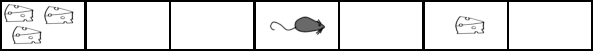
\includegraphics[width=8cm]{img/mouse_walk}
\captionof{figure}{The mouse can move one tile at a time to the \textbf{R}ight or to the \textbf{L}eft.}
\label{fig:mouse_walk}
\end{center}

% Please add the following required packages to your document preamble:
% \usepackage{graphicx}
\begin{table}[h]
\centering
\resizebox{0.7\textwidth}{!}{%
\begin{tabular}{lcrl}
\multicolumn{1}{c|}{strategy}   & \multicolumn{1}{c|}{$\gamma$}                       & return(1)                                                                  &                                                 \\ \hline \hline
                                %& \multicolumn{1}{l}{}                                & \multicolumn{1}{l}{}                                                       &                                                 \\ \hline
%\multicolumn{1}{|c|}{strategy}  & \multicolumn{1}{c|}{$\gamma$}      & return(1)                                                                  & \multicolumn{1}{l|}{}                           \\ \hline \hline
                                %& \multicolumn{1}{l}{}               & \multicolumn{1}{l}{}                                                       &                                                 \\ \hline
\multicolumn{1}{|l|}{R,R,...}   & \multicolumn{1}{c|}{\multirow{2}{*}{$\frac{1}{2}$}} & $\frac{1}{2} \cdot 0 + \frac{1}{4} \cdot 1 + \ldots$                       & \multicolumn{1}{l|}{$\ge {0.25}$}             \\   \cline{1-1} \cline{3-4}
\multicolumn{1}{|l|}{L,L,L,...} & \multicolumn{1}{c|}{}              & $\frac{1}{2} \cdot 0 + \frac{1}{4} \cdot 0 + \frac{1}{8} \cdot 3 + \ldots$ & \multicolumn{1}{l|}{$\ge \mathbf{0.375}$} \\ \hline
                                & \multicolumn{1}{l}{}               & \multicolumn{1}{l}{}                                                       &                                                 \\   \hline
\multicolumn{1}{|l|}{R,R,...}   & \multicolumn{1}{c|}{\multirow{2}{*}{$0.7$}}         & $0.7 \cdot 0 + 0.7^2 \cdot 1 + \ldots$                                     & \multicolumn{1}{l|}{$\ge {0.48}$}                 \\ \cline{1-1} \cline{3-4}
\multicolumn{1}{|l|}{L,L,L,...} & \multicolumn{1}{c|}{}         & $0.7 \cdot 0 + 0.7^2 \cdot 0 + 0.7^3 \cdot 3 + \ldots$                     & \multicolumn{1}{l|}{$\ge \mathbf{1.02}$}                 \\ \hline
                                & \multicolumn{1}{l}{}               & \multicolumn{1}{l}{}                                                       &                                                 \\ \hline
\multicolumn{1}{|l|}{R,R,...}   & \multicolumn{1}{c|}{\multirow{2}{*}{$0.2$}}         & $0.2 \cdot 0 + 0.2^2 \cdot 1 + \ldots$                                     & \multicolumn{1}{l|}{$\ge \mathbf{0.04}$}                  \\   \cline{1-1} \cline{3-4}
\multicolumn{1}{|l|}{L,L,L,...} & \multicolumn{1}{l|}{}              & $0.2 \cdot 0 + 0.2^2 \cdot 0 + 0.2^3 \cdot 3 +\ldots$              & \multicolumn{1}{l|}{$\ge {0.024}$}                \\ \hline
\end{tabular}%
}
\captionof{table}{Comparing returns for two strategies under different discount factors.}

\end{table}
}



\end{frame}

\begin{frame}

\question{Why do we discount future rewards? What criteria goes into choosing $\gamma$?}\\

\pause

\begin{itemize}
\item Uncertainty of the future
\item Imperfections in the model (we don't trust its decisions completely)
\item mathematically convenient, the sum does not explode
\item avoids $\infty$ returns due to possible cycles in our MDP
\item behavioral arguments (animals and humans seem to apply a similar discounting)\\
``A bird in the hand is worth two in the bush''
\item financially realistic (accounts for inflation)
\end{itemize}

\end{frame} 

\newpage

\subsection{The value function}


\definecolor{darkgreen}{rgb}{0,.5,0}
\definecolor{discount}{rgb}{.75,0,.75}
\definecolor{expect}{rgb}{0,.5,.5}
\definecolor{chain}{rgb}{.75,.5,0}

\begin{frame}\frametitle{\subsecname}

The (state) value function $\corresponds$ the expected sum of discounted future rewards

\question{What does the value function represent?}

\begin{itemize}
\item The long-term value of some state $\vec x$,
\item the expected return from starting in $\vec x^{(0)}$,
\item we have a preference for high expectations and MDPs maximize this quantity
\end{itemize}

\end{frame}

\begin{frame}\frametitle{\subsecname}

\mode<presentation>{
The value function $\corresponds$ the expected sum of discounted future rewards
}

For a fixed policy ${\color{policy}\pi}$:

	\only<1-4>{
	
	\begin{itemize}
		\item a \textbf{value function} measures the quality 
			of a policy $\pi$ in state $\vec x^{(0)}$
			\iitem{$V^\pi(\vec x^{(0)})$ is
				the {\em \visible<1->{{\color{expect}expected}} 
				\visible<2->{{\color{chain}{%
						\only<3>{\color{discount}}%
						\visible<3->{infinite} 
					}sum} of}
				\visible<3->{{\color{discount} discounted}} 
				\visible<2->{future}
				\visible<1->{{\color{reward}reward\visible<2->{s}}}}}
	\end{itemize}
	\only<1,3>{\vspace{1mm}}
	
	\begin{equation}
				V^\pi(\vec x^{(0)}) 
				\;\;=\;\; \visible<1->{{ \color{expect}	\E\bigg\lbrack }} 
					\visible<2->{{\color{chain}\sum_{t=0}^{
						\slidesonly{\only<2>{H}}%
						\only<3->{{\color{discount}\infty}}}}}
				\visible<3->{{\color{discount} \gamma^t} \,}
				{\color{reward} r(
					\slidesonly{\only<1>{{\color{black} \vec x^{(0)}}}}
					\only<2->{{\color{trans} \vec x^{(t)}}}, 
					{\color{policy}\vec a^{(\slidesonly{\only<1>{0}}\only<2->{t})}}
				) } 
				{ \color{expect}
					\,\bigg| \begin{array}{c}
							\scriptstyle {\color{policy}
								\vec a^{(\slidesonly{\only<1>{0}}\only<2->{t})} 
								\;\sim\; \pi(\cdot\,|\,
									\vec x^{(\slidesonly{\only<1>{0}}\only<2->{t})}) 
								}\;\;\;\\
							\visible<2->{{\color{trans}
								\scriptstyle \vec x^{(t+1)} \;\sim\; 
								P(\cdot \,|\, \vec x^{(t)}, \vec a^{(t)})
							}}
					\end{array}\kern-1ex 
					\bigg\rbrack
				} 
				\visible<3->{\,,\quad {\color{discount}\gamma \in \lbrack0, 1)} \,.}
	\end{equation}
	}
    \only<5>{
    \mode<presentation>{
    \begin{center}
		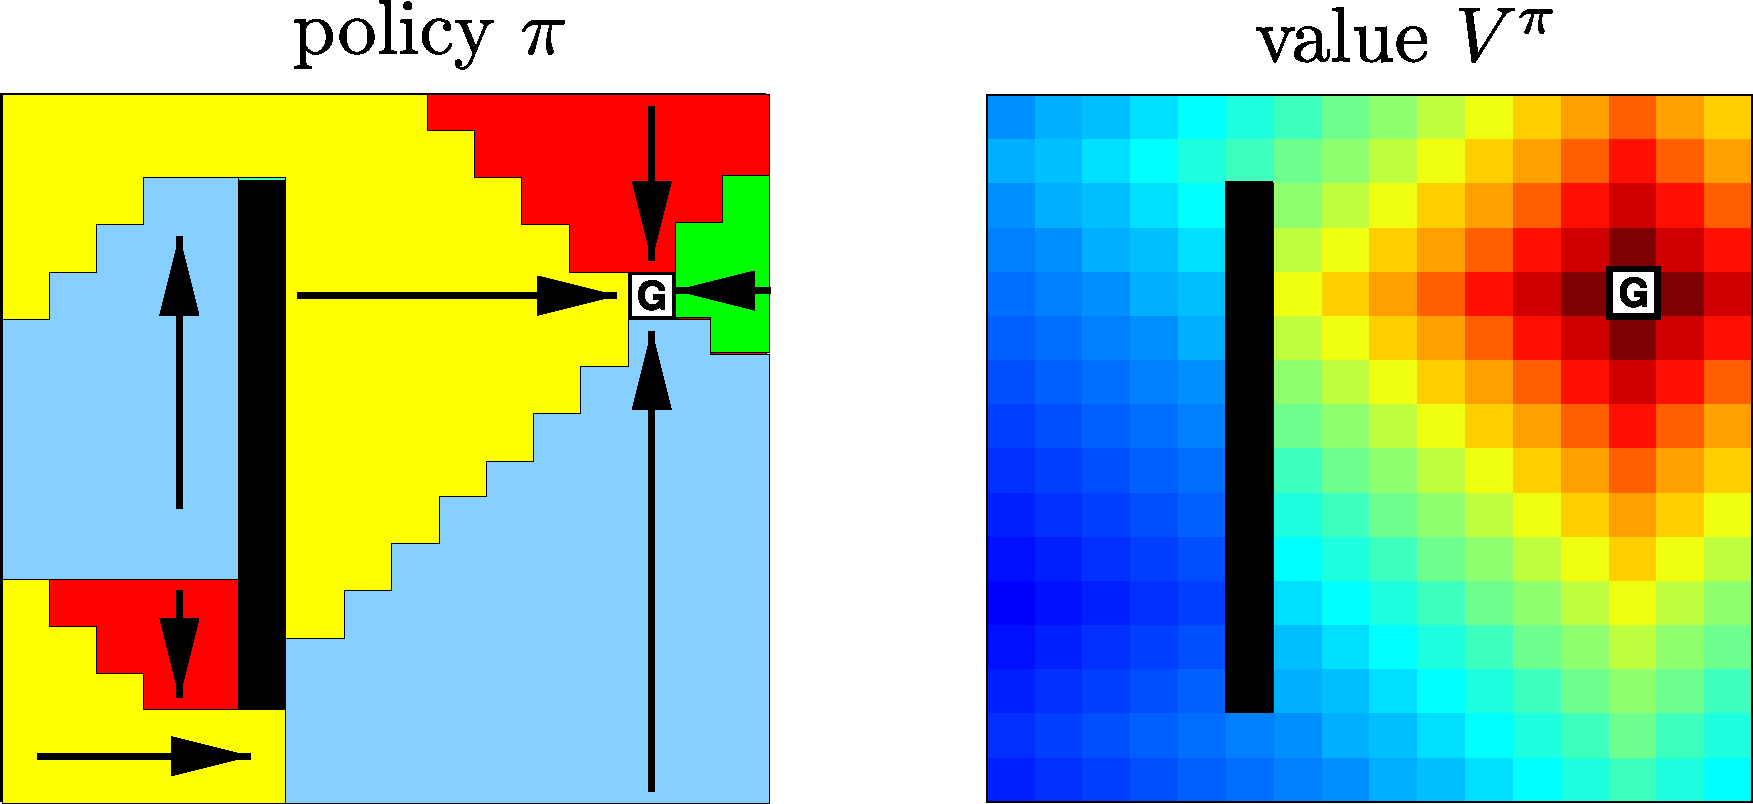
\includegraphics[trim={15cm 0 0 0mm},clip, height=3.cm]{img/nav_policy_and_value}
	\end{center}
    }
    }
    
    \visible<4,5>{
    
    
	In other textbooks you may find:
	
	\begin{align}
	V^\pi(\vec x_i) = \kern-1ex \overbrace{V^\pi_i}^{\text{shorthand}} \kern-1ex = 
	\E \bigg\lbrack
	\sum_{t=0}^{\infty} \gamma^t r(\vec x^{(t)}, \vec a^{(t)}) \;\Big|\; \vec x^{(0)} := \vec x_i
	\bigg\rbrack\,, \; i=1,\ldots,S
	\end{align}
	
	$\E\lbrack\cdot\rbrack$ is w.r.t $\{\vec x^{(t)}, \vec a^{(t)}\}$

    }

\end{frame}

\mode*

\clearpage

\mode<all>
\section{Model-based evaluation of the policy}

\begin{frame} 
\mode<presentation>{
    \begin{center} \huge
        \secname
    \end{center}  
    }
    \begin{center} 
    Model-based $\corresponds$ offline-planning.\\
    We are told everything about the environment,\\so we can simulate ``looking ahead'' and\\ determine if one policy is better than another.
    \end{center}
    
    \begin{center}
		
\includegraphics[width=0.3\textwidth]{img/meme_model-based}
    \end{center}
\end{frame}

\subsection{The Bellman equation}

\begin{frame}\frametitle{\subsecname}

The Bellman equation relates the value of a state with the values of its successor states, given some policy $\pi$.

The policy is fixed beforehand, i.e. $V$ ``follows'' the policy $\pi$.

\end{frame}

\begin{frame}\frametitle{\subsecname}


\slidesonly{\vspace{-4mm}}

	\begin{align}
	V^\pi_i 
    \only<1>{
    =\;&
	\E \Big\lbrack
	\sum_{t=0}^{\infty} \gamma^t \; \overbrace{r(\vec x^{(t)}, \vec a^{(t)})}^{\substack{\text{shorthand}\\=: r^{(t)}}} \;\Big|\; \vec x^{(0)} := \vec x_i
	\Big\rbrack\,, \; i=1,\ldots,S\\
	=\;& 
	\E \Big\lbrack
	\sum_{t=0}^{\infty} \gamma^t r^{(t)} \;\Big|\; \vec x^{(0)} := \vec x_i
	\Big\rbrack\\
	=\;& 
	\E \Big\lbrack
	\gamma^0 \kern-1.5ex \underbrace{r^{(0)}}_{\substack{\text{immediate}\\ \text{reward}}} \kern-1.5ex + \gamma^1 r^{(1)} + \gamma^2 r^{(2)}+\ldots\;\Big|\; \vec x^{(0)} := \vec x_i
	\Big\rbrack\\
	=\;& 
	\E \Big\lbrack
	r^{(0)} + 
	\underbrace{\gamma \big( r^{(1)} + \gamma r^{(2)}+\ldots\big)
	}_{\substack{
	\text{discounted value of}\\ \text{successor state}}}\;\Big|\; \vec x^{(0)} := \vec x_i
	\Big\rbrack\\}
    \only<1,2>{
	=\;&
	\E \Big\lbrack
	r^{(0)} + 
	\gamma V^\pi(\vec x^{(1)})\;\Big|\; \vec x^{(0)} := \vec x_i
	\Big\rbrack
    }
    \only<2>{
	\intertext{split ``expectation of sum'' into ``sum of expectations'':}
	=\;& 
	\E \Big\lbrack
	r^{(0)} \;\Big|\; \vec x^{(0)} := \vec x_i
	\Big\rbrack
	+
	\E \Big\lbrack
	{\color{red}\gamma} V^\pi( \vec x^{(1)})\;\Big|\; \vec x^{(0)} := \vec x_i
	\Big\rbrack\\
	=\;& 
	\E \Big\lbrack
	r^{(0)} \;\Big|\; \vec x^{(0)} := \vec x_i
	\Big\rbrack
	+
	{\color{red}\gamma}\,
	\E \Big\lbrack
	 V^\pi( \vec x^{(1)})\;\Big|\; \vec x^{(0)} := \vec x_i
	\Big\rbrack
    }
	\end{align}
	
\end{frame}

\begin{frame}\frametitle{\subsecname~(cont'd)}

\slidesonly{\vspace{-5mm}}

\mode<presentation>{
	\begin{align}
		V^\pi_i =\;& 
		\E \bigg\lbrack
		r^{(0)} \;\Big|\; \vec x^{(0)} := \vec x_i
		\bigg\rbrack
		+
		\gamma\,
		\E \bigg\lbrack
		 V^\pi( \vec x^{(1)})\;\Big|\; \vec x^{(0)} := \vec x_i
		\bigg\rbrack
	\end{align}

\only<1-3>{
Recall:
\begin{itemize}
\item[] states $\vec x \in \{ \vec x_1, \ldots, \vec x_S\}$, 
actions $\vec a \in \{ \vec a_1, \ldots, \vec a_A\}$,\\
reward function $r(\vec x_i, \vec a_k)$,
\item[]
transition model ${\color{trans} P(\vec x_j | \vec x_i, \vec a_k)}$ and
policy ${\color{policy} \pi(\vec a_k | \vec x_i)}$
\end{itemize}
}
}

\question{What does the $\E \lbrack \cdot \rbrack$ boil down to?}

\pause

\slidesonly{\vspace{-10mm}}

	\begin{align}
		V^\pi_i 
		&=& \visible<2->{
		\underbrace{
		{\color{policy} \sum_{k=1}^A \pi(\vec a_k \,|\, \vec x_i)}
			 {\color{reward} r(\vec x_i, \vec a_k)}
			 }_{\substack{\text{``controlled'' reward function }\\
			 \text{(immediate reward)} =: {\color{reward} r_i^\pi}}
			 }
		+
		}
		\visible<3->{
			 \underbrace{
			\gamma {\color{policy} \sum_{k=1}^A \pi(\vec a_k \,|\, \vec x_i)} {\color{trans}\smallsum{j=1}{S} 
				P(\vec x_j \,|\, \vec x_i, \vec a_k)} \kern-1.2ex
				\overbrace{V^\pi_j}^{=V^\pi(\vec x_j)}
				}_{\text{expected discounted value of successor state}} \\	
		&=& 
		}
		\visible<4->{
			\underbrace{{\color{policy} \smallsum{k=1}A 
				\pi(\vec a_k \,|\, \vec x_i)} 
				{\color{reward} r(\vec x_i, \vec a_k)}
			}_{\kern-4ex\text{``controlled'' reward function }
					{\color{reward} r_i^\pi}\kern-4ex}
			\;+\; \gamma {\color{trans} \smallsum{j=1}{S}}
			\underbrace{
				{\color{policy} \smallsum{k=1}A 
				\pi(\vec a_k \,|\, \vec x_i)} 
				{\color{trans} P(\vec x_j \,|\, \vec x_i, \vec a_k)}
			}_{\text{``controlled'' transition model }
					{\color{trans} P^\pi_{ij}}}  V^\pi_j
		}
	\end{align}
	
	\notesonly{
	Thus, the Bellman equation can be expressed using:
	
	\begin{equation}
	V^\pi_i
	= {\color{reward} r^\pi_i} 
			+ \gamma {\color{trans} P^\pi_{ij}} V^\pi_{j}
	\end{equation}
	}
	\visible<4>{
	
	\mode<presentation>{
		$$
		\vec v^\pi
		= {\color{reward}\vec r^\pi} 
				+ \gamma {\color{trans}\vec P^\pi} \vec v^\pi
		$$
		}
	}
	
	
\end{frame}

\begin{frame}

\notesonly{We can also use vector notation to represent the value of all states collectively:}
	
	\begin{equation}
		\vec v^\pi
		= \; {\color{reward}\vec r^\pi} 
			+ \gamma {\color{trans}\vec P^\pi} \vec v^\pi \; =: \kern-3ex\overbrace{\hat B^\pi[\vec v^\pi]}^{\text{the Bellman operator}}\kern-3ex,
	\end{equation}
	
	where $\vec v^\pi \in \R^S$ is a vector containing all values $V^\pi(\vec x_{i})\;\forall i$,
	
	\begin{align}
		\quad \text{with}  \underbrace{ \left\{ \begin{array}{rcl} 
				{\color{reward}r^\pi_i} &\kern-1ex:=\kern-1ex& 
					{\color{policy} \smallsum{k=1}{A} 
					\pi(\vec a_k \,|\, \vec x_i)} \, 
					{\color{reward} r(\vec x_i, \vec a_k)} \\
				{\color{trans}P^\pi_{ij}} &\kern-1ex:=\kern-1ex& 
					{\color{policy}\smallsum{k=1}{A} 
					\pi(\vec a_k \,|\, \vec x_i)} \, 
					{\color{trans}P(\vec x_j | \vec x_i, \vec a_k)} \\
			\end{array} 
			\right.\kern-2ex}_{
				\text{``controlled'' models }
				{\color{reward}\vec r^\pi \in \R^S}
				\text{ and }{\color{trans}\vec P^\pi \in \R^{S \times S}}
			}
	\end{align}
	
\end{frame}

\subsection{Finding the value}

\begin{frame}\frametitle{Finding $\vec v^\pi$}

\mode<presentation>{
	$$
	\vec v^\pi
	= {\color{reward}\vec r^\pi} 
			+ \gamma {\color{trans}\vec P^\pi} \vec v^\pi
	$$
	
}
There are two approaches to finding $\vec v^\pi$:

\begin{enumerate}
\item[\ref{sec:findvanalytical} -] analytically
\item[\ref{sec:findviter} -] through fixed-point iteration
\end{enumerate}

\end{frame}

\subsubsection{Analytical solution of the Bellman equation}\label{sec:findvanalytical}

\begin{frame}\frametitle{Finding $\vec v^\pi$:~\subsubsecname}

Essentially solve for $\vec v^\pi$ (get \underline{all} $\vec v^\pi$ on one side):

\svspace{-5mm}

	\begin{align}
		\vec v^\pi &= {\color{reward}\vec r^\pi} 
		+ \gamma {\color{trans}\vec P^\pi} \vec v^\pi \\
		\vec I~\vec v^\pi 
        &= {\color{reward}\vec r^\pi}
		+ \gamma {\color{trans}\vec P^\pi} \vec v^\pi
	\\
		\vec I~\vec v^\pi - \gamma {\color{trans}\vec P^\pi} \vec v^\pi
		&= {\color{reward}\vec r^\pi}
	\\
		\big(\vec I - \gamma {\color{trans}\vec P^\pi}\big) \vec v^\pi
		&= {\color{reward}\vec r^\pi}
	\\
	\vec v^\pi &= \big(\vec I 
			- \gamma {\color{trans}\vec P^\pi}\big)^{-1}
		 {\color{reward}\vec r^\pi}
	\end{align}
	
	\question{When is the term $\big(\vec I 
			- \gamma {\color{trans}\vec P^\pi}\big)$ invertible?}
		
\begin{enumerate}
\item $|\lambda_k| \leq 1$ for all eigenvalues 
				$\lambda_k$ of transition matrix ${\color{trans}\vec P^\pi}$
\item $\gamma < 1$
\item[$\Rightarrow$] it is always invertible
\end{enumerate}

\end{frame}

\begin{frame}\frametitle{Finding $\vec v^\pi$:~\subsubsecname}

%\pause

%\svspace{-5mm}

\mode<presentation>{
\begin{equation}
	\vec v^\pi = \big(\vec I 
			- \gamma {\color{trans}\vec P^\pi}\big)^{-1}
		 {\color{reward}\vec r^\pi}
\end{equation}
}

\question{Any disadvantages to the analytical solution?}\\

\mode<presentation>{
\only<1>{
\begin{center}
	
\includegraphics[width=0.2\textwidth]{img/meme_analyticalbest}
\end{center}
}
\only<2>{
\begin{center}
\begin{minipage}{.3\textwidth}
\begin{center}
	
\includegraphics[width=0.9\textwidth]{img/meme_statespacetoobig}
\end{center}
\end{minipage}
\begin{minipage}{.3\textwidth}
\begin{center}
	
\includegraphics[width=0.8\textwidth]{img/meme_canthandleanalytical}
\end{center}
\end{minipage}
\end{center}
}
}

\pause 
- It could be very costly for very large state spaces.

\end{frame}


\subsubsection{Value iteration}\label{sec:findviter}

\begin{frame}\frametitle{Finding $\vec v^\pi$:~\subsubsecname}

Value iteration: a fixed-point iteration for finding $\vec v^\pi$

\begin{itemize}
\item A fixed point: $x=g(x)=g(g(\ldots g(x)\ldots))$\\

Example:
\svspace{-3mm}
\begin{align}
    g(x) &= x^{2} - 3x + 4\\
    g(2) &= 2^{2} - 3\cdot 2 + 4 = 4 - 6 + 4 = 2
\end{align}

\item Fixed point iteration:
\begin{equation}
x^{(t+1)} = g(x^{(t)}), t=0,1,2,\ldots
\end{equation}
\end{itemize}

\begin{center}
    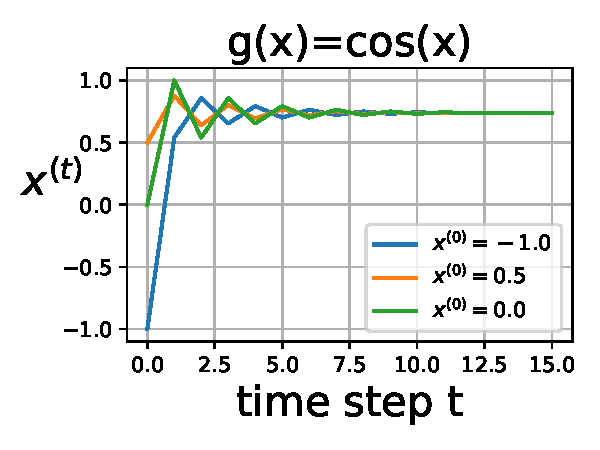
\includegraphics[height=3.5cm]{img/fixed_point_iter_cos} 
    \mode<article>{
    \captionof{figure}{
    Fixed point iteration example
    }
    \label{fig:fixedpointcos}
    } 
\end{center}

\mode<presentation>{
\only<2>{
	\placeimage{11.5}{9.3}{img/meme_fixedpoint}{width=3.5cm}
}
}

\end{frame}


\begin{frame}\frametitle{Finding $\vec v^\pi$:~\subsubsecname}
\mode<presentation>{
Value iteration: a fixed-point iteration for finding $\vec v^\pi$
}

\begin{equation}
	\vec {\tilde v}^{\pi (t+1)} = {\color{reward}\vec r^\pi} 
		+ \gamma {\color{trans}\vec P^\pi} \vec {\tilde v}^{\pi (t)} 
\end{equation}

\begin{itemize}
\item 
The ``~$\tilde{}$~'' is to denote that it has not necessarily converged 
at time step $t$
\item initialize $\vec {\tilde v}^{\pi (0)}$ with some state $\vec {\tilde v}^{\pi (0)} \in \R^{S}$
\item value iteration converges in the limit $t \rightarrow \infty$
\item The speed of convergence depends on $\gamma$
\end{itemize}

\question{How does convergence depend on $\gamma$?}

\pause 

\begin{itemize}
\item small $\gamma$: fast convergence
\item $\gamma \rightarrow 1$: slow convergence, slower than the analytical solution
\end{itemize}

\end{frame}


\begin{frame}\frametitle{Finding $\vec v^\pi$:~\subsubsecname}
    
\mode<presentation>{
\begin{equation}
	\vec {\tilde v}^{\pi (t+1)} = {\color{reward}\vec r^\pi} 
		+ \gamma {\color{trans}\vec P^\pi} \vec {\tilde v}^{\pi (t)} 
\end{equation}
}

\begin{itemize}
\item We start \emph{value iteration} assuming $\vec {\tilde v}^{\pi (0)}$ is the optimal value function
\item Use the one-step \emph{look-ahead} (i.e. next step) to work our way \emph{backwards}\\

	\begin{equation*}
		\hat B^\pi[\vec v^\pi] :=
		{\color{reward}\vec r^\pi} 
			+ \gamma {\color{trans}\vec P^\pi} \kern-2.7ex \underbrace{\vec v^\pi}_{\text{look-ahead}}
	\end{equation*}
\end{itemize}

\end{frame}

\begin{frame}\frametitle{Analytical solution vs. value iteration}

\mode<article>{
Analytical solution vs. value iteration:
}

\begin{itemize}
\item complexity: 
\begin{itemize}
\item Analytical solution: $O(S^{3})$
\item value iteration: $O(S^{2})$
\end{itemize}   
\item intermediate solutions of \emph{value iteration} don't necessarily belong to valid policies. We have to wait for convergence.
\end{itemize}

\end{frame}

\newpage

%\subsubsection{Convergence of value iteration}
% excluded

% -----------------------------------------------------------------------------
%\begin{frame} \frametitle{\subsubsecname}
    
    %\only<1,2>{
	%\begin{block}{Contraction mapping}
		%\small
		%A mapping function $f(x)$ is a contraction with $0 < \gamma < 1$ if for any $x, x'$, $\lVert f(x) - f(x') \rVert \le \gamma \lVert x - x' \rVert$.
	%\normalsize
	%\end{block}
    
    %\mode<article>{
    %We specify this a little further:
    %}
    %}
    
    %\only<2->{
	%\begin{block}{Contraction mapping (in supremum norm)}
		%\small
		%A function $\hat B : \R^S \to \R^S$ is called a 
		%{\em contraction mapping} 
		%with Lipschitz constant\notesonly{\footnote{i.e. the function is continuous and the absolute value of the slope does not exceed some constant, which is a real number. That real number is the Lipschitz constant.}} $0 \leq \lambda < 1$ if 
		%$\max\limits_{j} 
		%\big|(\hat B[\tilde{\vec v}] - \hat B[\tilde{\vec w}])_j \big| 
		%\;\leq\; \lambda \max\limits_{j} \big|\tilde v_j - \tilde w_j \big|,
		%\forall \tilde{\vec v}, \tilde{\vec w} \in \R^S$.
	%\normalsize
	%\end{block}
	%}
	%\only<3>{ 
		%\vspace{2mm}
		%\iitem{application to the Bellman operator 
				%$\hat B^\pi[\tilde{\vec v}] =
				%{\color{reward}\vec r^\pi} 
				%+ \gamma {\color{trans}\vec P^\pi} \tilde{\vec v}$}
		%\begin{eqnarray*}
			%\max_j \big| \hat B^\pi[\tilde{\vec v}]_j 
				%- \hat B^\pi[\tilde{\vec w}]_j \big| 
			%&=& \max_j
				%\big| {\color{reward} r^\pi_j} 
					%+ \gamma {\color{trans}(\vec P^\pi \tilde{\vec v})_j}
					%- {\color{reward}r^\pi_j} 
					%- \gamma {\color{trans}(\vec P^\pi \tilde{\vec w})_j} 
				%\big| \\[-2mm]
			%&\stackrel{\text{(i)}}{\leq}& 
				%\max_j \gamma \, \big({\color{trans}\vec P^\pi} 
				%|\tilde{\vec v} - \tilde{\vec w}|\big)_j 
			%\quad\stackrel{\text{(ii)}}{\leq}\quad  
				%\gamma \, \max_j |\tilde v_j - \tilde w_j|
		%\end{eqnarray*}
		%\vspace{2mm}
		%\begin{eqnarray*}
			%\text{(i)} \quad 
			 %\Big|{\color{trans}\smallsum{i=1}{S} P^\pi_{ji}} \,x_i \Big|
			 	%&\leq & 
				 %{\color{trans} \smallsum{i=1}{S} P^\pi_{ji}} \, |x_i| \,,
				 %\qquad\; \forall \vec x \in \R^S 
				 %\hspace{1.2cm}\text{(Jensen's inequality)} \\[-1mm]
			%\text{(ii)} \quad
			%{\color{trans}\smallsum{i=1}{S} P^\pi_{ji}} \, |x_i|
				%& \leq &
				%{\color{trans} \smallsum{i=1}{S} P^\pi_{ji}}
					%\max_{1\leq k\leq S} |x_k|
				%\quad = \;\;\; \max_{1\leq k\leq S} |x_k| 
				%\hspace{1.1cm}
				%\text{(${\color{trans}\smallsum{i=1}{S} P^\pi_{ji} = 1}$)}
		%\end{eqnarray*}
	%} \only<4>{
		%\vspace{1mm}
		%\begin{itemize}
			%\item $\hat B^\pi$ is a contraction mapping 
				%with Lipschitz constant $0 < \gamma < 1$ 
			%\vspace{2mm}
			%\begin{align} \tag{value iteration}
				%\tilde{\vec v}^{\pi(t+1)} 
				%\quad=\quad \hat B^\pi\lbrack\tilde{\vec v}^{\pi(t)}]\rbrack
				%\quad=\quad {\color{reward}\vec r^\pi} 
					%+ \gamma {\color{trans}\vec P^\pi} \tilde{\vec v}^{\pi(t)}
			%\end{align}
			%\vspace{-2mm}
			%\item Let $\vec v^\pi$ be the unique fixed point. Then:\\[10pt]
			%\hspace{-3mm}$\max\limits_j \big|
				%(\hat B^\pi \lbrack \vec v^{\pi(t)} \rbrack)_j - (\hat B^\pi \lbrack \vec v^{\pi} \rbrack)_j \big| 
				%\leq \gamma \max\limits_j 
					%\big|v^{\pi(t)}_j - v^\pi_j \big| $ 
				%for {\em any} $\vec v^{\pi(t)} \in \R^S$
			%\vspace{1mm}
			%\item[$\Rightarrow$] value iteration converges in the limit $t\to\infty$
				%\vspace{1mm}
				%\iitem{number of iterations until convergence 
					%$\sim -\frac{1}{\log(\gamma)}$
				 %\vspace{1mm}
				 %\item analytic solution is faster for large values of $\gamma$
				%}
		%\end{itemize} 
		%\vspace{4mm}
	%}
%\end{frame}

\newpage

\subsection{Finding the optimal policy}

\subsubsection{Comparing two policies}

\mode<presentation>{
\begin{frame}    
	\begin{center} \LARGE
        \subsecname
    \end{center}      
	\begin{center}
        \subsubsecname
    \end{center}  
\end{frame}
}

\begin{frame}\frametitle{My policy is better than yours}

\notesonly{
A policy $\pi$ is regarded as better or equal to another policy $\pi'$ if $\pi$ yields an expected return which is greater or equal to that of the other policy $\pi'$ for all possible states.
That is,
}

\begin{equation}
\pi~
\overset{\mathclap{\substack{%
					\text{``better'' or}\\[1mm]\text{equally ``good''}\\ \big\downarrow
					}}}{{\color{gray}\ge}}
~\pi' 
\quad \text{\textbf{iff}} \quad V^{\pi} (\vec x) \ge V^{\pi'} (\vec x)\,,\quad \forall\; \vec x \in \mathcal{X}
\end{equation}

\end{frame}

\begin{frame}\frametitle{\subsecname}

Multiple \emph{optimal policies} can exist. A policy is optimal if it maximizes the state value function\notesonly{\footnote{For more information, see Ch 3.6 in \citep{sutton1998introduction}}}:

\begin{equation}
V^{*}(\vec x) = \max_{\pi} V^{\pi} (\vec x)\,,\quad \forall\; \vec x \in \mathcal{X}
\end{equation}

\begin{block}{Optimal Policy}

For all optimal policies $\pi^{*}$:

\begin{equation}
    V^{\pi^{*}}(\vec x) = V^{*}(\vec x) 
\end{equation}

A policy $\pi$ that maximizes the value function and yields $\vec v^{*}$ is an optimal policy $\pi^{*}$.
    
\end{block}

    
\end{frame}

\subsection{Extracting the policy from an optimal value function}

\begin{frame}\frametitle{\subsecname}

\slidesonly{\vspace{-3mm}} 

\begin{center}
    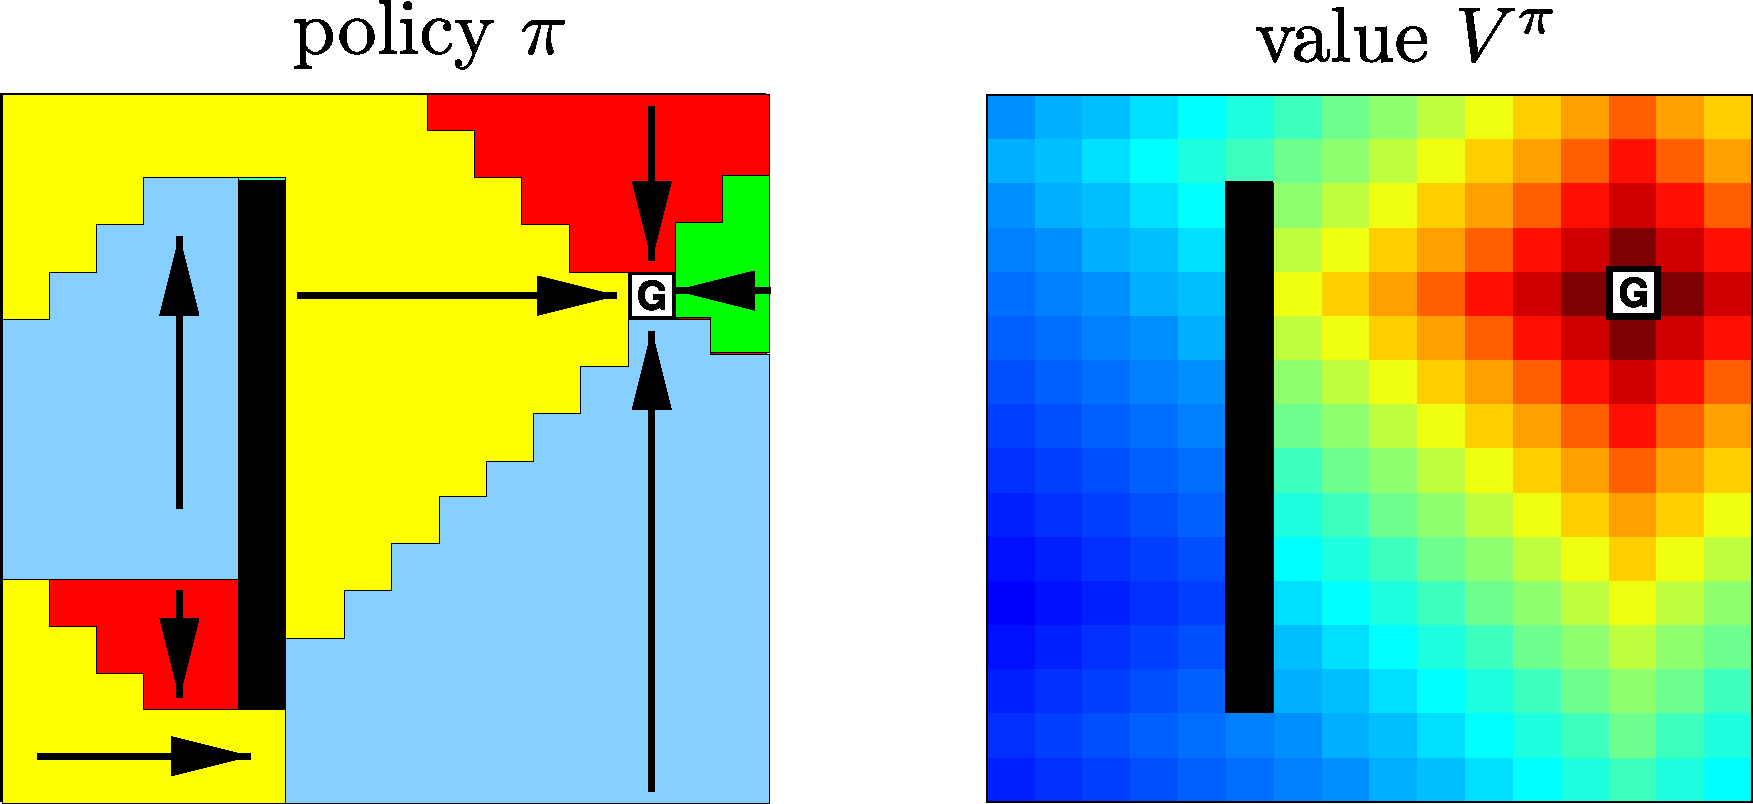
\includegraphics[trim={15cm 0 0 0mm},clip, height=3.5cm]{img/nav_policy_and_value} 
    \mode<article>{
    \captionof{figure}{
    Extract optimal policy from optimal value function
    }
    \label{fig:selectoptimalpolicy}
    } 
\end{center}

\pause

\slidesonly{\vspace{-5mm}}

\begin{equation}
\pi^{*}(\vec a_{k} | \vec x_{i}) = \argmax_{\vec a} \Big( {\color{reward}r(\vec x_{i}, \vec a)} +  \gamma \sum_{j=1}^{S} {\color{trans} P(\vec x_{j}| \vec x_{i}, \vec a)} V^{*}(\vec x_{j}) \Big)    
\end{equation}   

\slidesonly{\vspace{-5mm}} 

\only<3>{
\question{What is going on here?}

\begin{enumerate}
%\item An optimal policy selects the action that maximizes this 
\item When at $\vec x_{i}$, look at the actions $\vec a$ that lead to all possible future states $\vec x_{j}$.
\item Select action $\vec a_{k}$ that maximizes the immediate reward + discounted successive value.
\end{enumerate}
}

\only<4>{
\question{What are the implications of selecting the optimal policy this way?}

\begin{itemize}
\item The above does not scale well for large state spaces.
\item The resulting $\pi^{*}$ is a \emph{greedy} policy, because it greedily selects using only the value function at hand. 
\end{itemize}
}

\end{frame}

\mode*

%\clearpage

\section{References}
\begin{frame}[allowframebreaks] \frametitle{References}
	\scriptsize
	\bibliographystyle{plainnat}
	\bibliography{bibliography}
\end{frame}

\end{rightcolumn}
\end{paracol}

\end{document}
